\newpage
\subsubsection{Programmflussdiagramm}
\label{subsubsec:Programmflussdiagramm}

\paragraph{Bootloader-Section}\mbox{}\\
In Abbildung \ref{fig:Programmfluss_Atmega2560} wird der Programmfluss der Mikrocontroller-Software aufgezeigt. Beim einschalten des Mikrocontrollers wird in der Bootloader-Section zuerst der Bootloader gestartet (Boot Loader Flash Section). Sofern keine neue Software über die UART0-Schnittstelle kommt, so beginnt das Cocktail spezifische Programm (Application Flash Section). Sofern eine neue Software über die UART0-Schnittstelle gesendet wird, wird die kommende Software in diese Application Flash Section geschrieben und das Programm nach der Übertragung gestartet.

\paragraph{Init-Section}\mbox{}\\
Wird das Programm gestartet, beginnt die Init-Section. Hier werden die zuerst die Main-Variablen initialisiert. Danach werden die Adressen der Funktionen ins Programm geladen mittels den h-Files. Die Interfaces (SPI, Uart, I/O's) müssen als erstes initialisiert werden, damit die Initialisierung der SPI-Devices stattfinden kann und Boot-Informationen über eine gewünschte Schnittstelle angezeigt werden können (z.B Uart0 ==> Computer). Sobald die Schnittstellen initialisiert wurden, werden die Devices initialisiert. Dazu gehören die SD-Karte, der FOC-Treiber und der Gate-Treiber. Daraufhin werden die Speicher-Strukturen initialisiert, welche für die User-Applikation (Tabelle \ref{fig:Softwareuebersicht_Atmega2560} in Kapitel \ref{subsubsec:Strukturplan_Atmega}) gebraucht werden. Zu guter Letzt wird die Startanzeige des Displays geladen.

\paragraph{Main-Loop}\mbox{}\\
Da die Maschine nur auf Inputs reagieren muss, werden im Main-Loop nur die Buffer der Devices abgefragt. Sobald ein Terminator-Zeichen ankommt (z.B ein carriage return '\textbackslash r' der UART0-Schnitstelle oder 0xFF 0xFF 0xFF der UART1-Schnittstelle), werden die zuvor empfangenen Daten interpretiert und verarbeitet.

\begin{figure}[H]
	\centering
	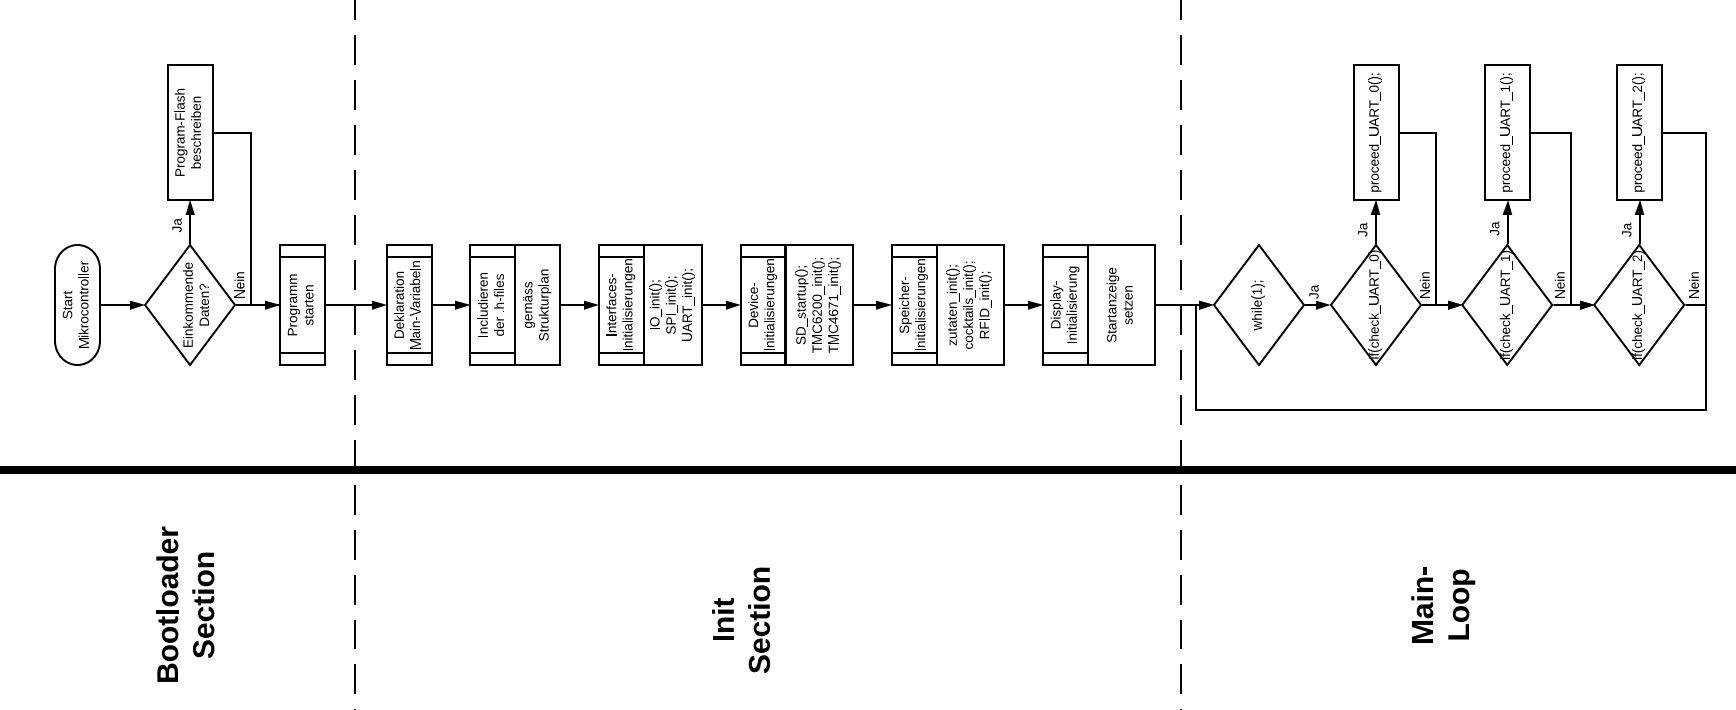
\includegraphics[angle = 270, width=0.6\textwidth]{graphics/ProgrammflussMikrokontroller}
	\caption{Programmfluss Mikrocontroller}
	\label{fig:Programmfluss_Atmega2560}
\end{figure}

\subsubsection{Speicherorganisation}\label{subsubsec:Speicherorganisation}

Da im Programmfluss viel mit Listen gearbeitet wird, wird auf \textit{Doubly Dynamic Linked Lists} zurückgegriffen.
Eine Doppelt verkettete Liste ist eine gängige Datenstruktur, um sich einfach und effizient in einer Liste hoch und runter zu bewegen. Weiter können der Liste ohne grossen Aufwand sogenannte Nodes\footnote{Nodes = Knoten} hinzugefügt werden. Im Folgenden wird von Elementen statt von Nodes gesprochen. Für jedes Element werden zwei Pointer initialisiert, welche auf das nächste (next) oder auf das vorherige (prev) Element zeigen. Nebst den Pointern auf die umliegenden Elemente enthält das Element die gewünschten Daten. Um zu wissen, ob das Ende oder der Beginn erreicht wurde, werden zwei zusätzliche Pointer initialisiert, welche auf das erste und/oder letzte Element zeigen (Head und Tail).
%Im Anhang Kapitel \ref{Appendix:Lists} können weitere Details zu Dynamic Linked Lists entnommen werden.
Abbildung \ref{fig:Doubly_Linked_List_2_00} zeigt eine Struktur der beschriebenen Liste mit next, prev, head, tail und Elementen. \cite{lenz_artikel_2016}

\begin{figure}[h!]
	\centering
	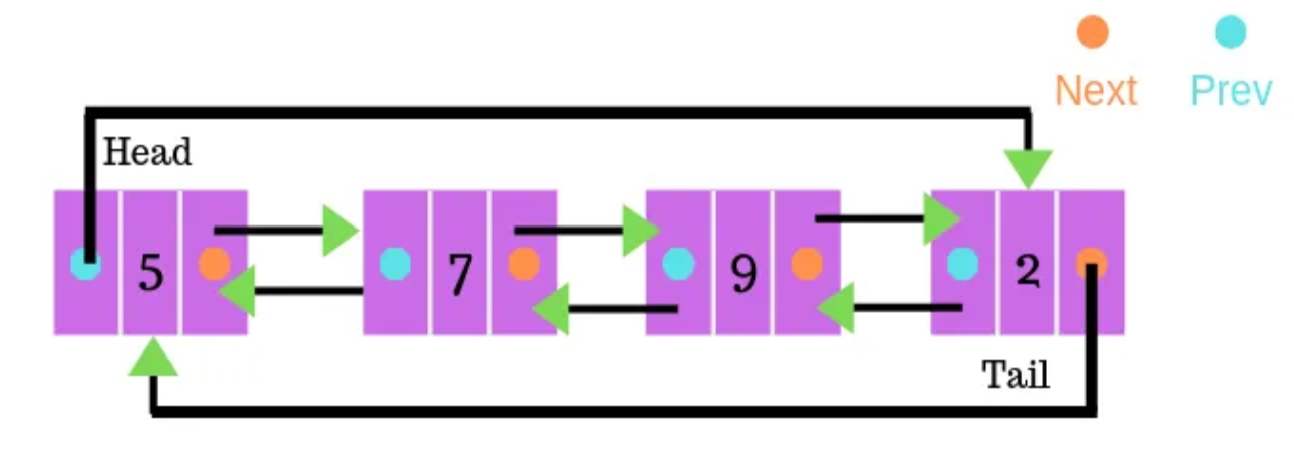
\includegraphics[width=0.5\textwidth]{graphics/Doubly_Linked_List_2_00}
	\caption{Doppelt verkettete Liste mit zwei Elementen.\cite{yadav_circular_2019}}
	\label{fig:Doubly_Linked_List_2_00}
\end{figure}


Die Elemente sind in Structs organisiert, welche die Pointer und die Daten enthalten. In der Software werden verschiedene Struct-Typen verwendet. Für jeden Struct-Typ lässt sich eine Liste mit mehreren Structs erstellen. Es werden für die folgenden fünf Elemente Listen angelegt:

\begin{itemize}
\item Cocktail-Liste (SD-Files)
\item Zutaten-Liste (SD-Files)
\item Tag-Liste (Maschine)
\item Zutaten-in-Maschine-Liste (Maschine)
\item Listen-Pointer
\end{itemize}

Die Cocktail- und die Zutaten-Liste beinhalten nur die Nummer eines zugehöriges Files, welches sich auf der SD-Karte befindet. Wird ein Cocktail oder eine Zutat benötigt, so werden die Daten temporär von der SD-Karte in einen Struct im Programmspeicher geladen und überschrieben, sobald eine andere Zutat oder ein anderer Cocktail geladen wird.

Die Cocktails sind folglich separat gepseichert, genauso die Zutaten. Die Liste, welche Informationen zu den Zutaten in der Maschine beinhaltet, wird als ein einziges File auf der SD-Karte gespeichert.